\renewcommand{\thesection}{\arabic{section}}\renewcommand{\theHsection}{chapter.\arabic{section}}\setcounter{section}{0}\section{群}
\noindent\begin{minipage}{\textwidth}\ProblemHeading{例题}{1.1（改写）}
用模 $2$ 的同余关系，将偶数集合 $\{0,\pm2,\pm4,\ldots\}$ 用描述法表示。
\end{minipage}\par\vfill
\noindent\begin{minipage}{\textwidth}\ProblemHeading{例题}{1.2（改写）}
设 $A$ 是集合。定义恒等映射 $1_A:A\to A$，其中 $1_A(a)=a$。证明 $1_A$ 是一一对应。
\end{minipage}\par\vfill
\noindent\begin{minipage}{\textwidth}\ProblemHeading{习题}{1.3}
设 $\sim$ 是集合 $A$ 上的等价关系。对 $a\in A$，令 $[a]=\{b\in A\mid b\sim a\}$。证明 $A$ 上的不同等价类互不相交。
\end{minipage}\par\vfill
\newpage
\noindent\begin{minipage}{\textwidth}\ProblemHeading{习题}{1.4}
设 $\{A_i\mid i\in I\}$ 是集合 $A$ 的一个分拆，即 $A=\bigcup_{i\in I}A_i$，且各个 $A_i$ 两两不相交。对 $a,b\in A$，规定 $a\sim b$ 当且仅当 $a,b$ 属于同一个 $A_i$。证明 $\sim$ 是 $A$ 上的等价关系。
\end{minipage}\par\vfill
\noindent\begin{minipage}{\textwidth}\ProblemHeading{例题}{1.5（改写）}
设 $F$ 是由若干集合构成的集族。对 $A,B\in F$，规定 $A\sim B$ 当且仅当存在从 $A$ 到 $B$ 的一一对应。证明 $\sim$ 是 $F$ 上的等价关系。
\end{minipage}\par\vfill
\noindent\begin{minipage}{\textwidth}\ProblemHeading{例题}{1.6（改写）}
设 $A,B$ 是有限集。证明 $A$ 与 $B$ 之间存在一一对应，当且仅当 $|A|=|B|$。
\end{minipage}\par\vfill
\newpage
\noindent\begin{minipage}{\textwidth}\ProblemHeading{例题}{1.7（改写）}
设 $E$ 是全体正偶数构成的集合。证明 $E$ 可数无限，并由此说明无限集合可以与它的一个真子集等势。
\end{minipage}\par\vfill
\noindent\begin{minipage}{\textwidth}\ProblemHeading{习题}{1.8}
设 $B$ 和 $A_i$（$i\in I$）均为同一全集 $\Omega$ 的子集，补集均在 $\Omega$ 中取。证明：
\SubQ{1}{$B\cap\left(\bigcup_{i\in I}A_i\right)=\bigcup_{i\in I}(B\cap A_i)$。}
\SubQ{2}{$B\cup\left(\bigcap_{i\in I}A_i\right)=\bigcap_{i\in I}(B\cup A_i)$。}
\SubQ{3}{$\overline{\bigcup_{i\in I}A_i}=\bigcap_{i\in I}\overline{A_i}$，且 $\overline{\bigcap_{i\in I}A_i}=\bigcup_{i\in I}\overline{A_i}$。}
\end{minipage}\par\vfill
\noindent\begin{minipage}{\textwidth}\ProblemHeading{习题}{1.9}
设 $f:A\to B$ 是集合之间的映射，$A$ 非空，$1_A$ 与 $1_B$ 分别表示相应集合的恒等映射。证明：
\SubQ{1}{$f$ 是单射，当且仅当存在 $g:B\to A$，使得 $g\circ f=1_A$。}
\SubQ{2}{$f$ 是满射，当且仅当存在 $h:B\to A$，使得 $f\circ h=1_B$。}
\end{minipage}\par\vfill
\newpage
\noindent\begin{minipage}{\textwidth}\ProblemHeading{习题}{1.10}
设 $f:A\to B$ 与 $g:B\to C$ 均为一一对应。证明 $g\circ f:A\to C$ 也是一一对应，且 $(g\circ f)^{-1}=f^{-1}\circ g^{-1}$。
\end{minipage}\par\vfill
\noindent\begin{minipage}{\textwidth}\ProblemHeading{习题}{1.11}
设 $A$ 是有限集，$P(A)$ 是由 $A$ 的全部子集（包括空集）构成的集族。证明 $|P(A)|=2^{|A|}$。
\end{minipage}\par\vfill
\noindent\begin{minipage}{\textwidth}\ProblemHeading{习题}{1.12}
设 $f:A\to B$ 是集合之间的映射。对任意 $a,a'\in A$，规定 $a\sim a'$ 当且仅当 $f(a)=f(a')$。证明 $\sim$ 是 $A$ 上的等价关系。
\end{minipage}\par\vfill
\newpage
\noindent\begin{minipage}{\textwidth}\ProblemHeading{习题}{1.13}
证明等价关系的自反性、对称性和传递性彼此独立，即任意两个条件都不能推出第三个条件。
\end{minipage}\par\vfill
\noindent\begin{minipage}{\textwidth}\ProblemHeading{习题}{1.14}
设 $A,B$ 是两个有限集合。
\SubQ{1}{从 $A$ 到 $B$ 的不同映射共有多少个？}
\SubQ{2}{$A$ 上的不同二元运算共有多少个？}
\end{minipage}\par\vfill
\noindent\begin{minipage}{\textwidth}\ProblemHeading{例题}{1.15（改写）}
设 $M$ 为全体非负整数，$\mathbb{Q}^{*}$、$\mathbb{R}^{*}$、$\mathbb{C}^{*}$ 分别为非零有理数、非零实数和非零复数全体。考察它们在下列运算下的结构。
\SubQ{1}{证明 $(M,+)$ 是含幺交换半群，确定其幺元素及全部可逆元素，并判断它是否是群。}
\SubQ{2}{判断 $\mathbb{Z}$、$\mathbb{Q}$、$\mathbb{R}$、$\mathbb{C}$ 对加法是否形成阿贝尔群。}
\SubQ{3}{判断正整数全体及 $\mathbb{Q}^{*}$、$\mathbb{R}^{*}$、$\mathbb{C}^{*}$ 对乘法分别是否形成含幺半群或阿贝尔群，并说明 $\mathbb{Q}^{*}$ 中元素的乘法逆。}
\end{minipage}\par\vfill
\newpage
\noindent\begin{minipage}{\textwidth}\ProblemHeading{例题}{1.16（改写）}
令 $M_{m,n}(\mathbb{C})$ 为全体 $m\times n$ 复矩阵组成的集合，$M_n(\mathbb{C})$ 为全体 $n$ 阶复方阵组成的集合，$m,n$ 为正整数。
\SubQ{1}{证明 $M_{m,n}(\mathbb{C})$ 对矩阵加法形成阿贝尔群，写出其幺元素以及矩阵 $A=(a_{ij})$ 的加法逆。}
\SubQ{2}{证明 $M_n(\mathbb{C})$ 对矩阵乘法形成含幺半群，写出幺元素，并用行列式刻画其中的可逆元素。}
\SubQ{3}{判断 $M_n(\mathbb{C})$ 对矩阵乘法是否为群。当 $n\geq 2$ 时，判断该乘法是否交换。}
\end{minipage}\par\vfill
\noindent\begin{minipage}{\textwidth}\ProblemHeading{例题}{1.17（改写）}
设 $A$ 为非空集合，$\Sigma(A)$ 为从 $A$ 到自身的全体映射组成的集合。
\SubQ{1}{证明 $\Sigma(A)$ 对映射的合成形成含幺半群，并写出其幺元素。}
\SubQ{2}{刻画 $\Sigma(A)$ 中可逆的映射。}
\SubQ{3}{当 $A$ 至少含两个元素时，证明 $\Sigma(A)$ 既不是群，其合成运算也不满足交换律。}
\end{minipage}\par\vfill
\noindent\begin{minipage}{\textwidth}\ProblemHeading{例题}{1.18（改写）}
把欧氏平面 $\mathbb{R}^{2}$ 中保持欧氏距离的映射称为欧氏运动。
\SubQ{1}{证明任何欧氏运动都是 $\mathbb{R}^2$ 到自身的双射，其逆映射也是欧氏运动。}
\SubQ{2}{证明平面上全体欧氏运动对映射合成形成群。}
\SubQ{3}{证明该群不是阿贝尔群。}
\end{minipage}\par\vfill
\newpage
\noindent\begin{minipage}{\textwidth}\ProblemHeading{例题}{1.19（改写、校订）}
设 $n$ 为正整数，在 $\mathbb{Z}$ 上定义 $a\sim b$ 当且仅当 $n\mid(a-b)$。记 $\overline{a}$ 为 $a$ 所在的等价类，$\mathbb{Z}_n$ 为全体等价类组成的集合。
\SubQ{1}{证明 $\sim$ 是等价关系，并给出一个完全代表系。}
\SubQ{2}{证明 $\overline{a}+\overline{b}=\overline{a+b}$ 与代表元的取法无关，且使 $\mathbb{Z}_n$ 成为阿贝尔群。}
\SubQ{3}{证明 $\overline{a}\,\overline{b}=\overline{ab}$ 与代表元的取法无关，且使 $\mathbb{Z}_n$ 成为含幺交换半群。用 $a$ 与 $n$ 的最大公因数刻画 $\overline{a}$ 的乘法可逆性。}
\end{minipage}\par\vfill
\noindent\begin{minipage}{\textwidth}\ProblemHeading{例题}{1.20（改写）}
设 $n$ 为正整数。对下述三种集合，验证它们在指定运算下形成群。
\SubQ{1}{全体 $n$ 阶可逆复方阵组成的集合 $\operatorname{GL}(n,\mathbb{C})$，运算为矩阵乘法。}
\SubQ{2}{非空集合 $A$ 到自身的全体双射组成的集合 $S(A)$，运算为映射合成。}
\SubQ{3}{模 $n$ 同余类中与 $n$ 互素的类组成的集合 $\mathbb{Z}_n^{*}=\{\overline{a}\mid\gcd(a,n)=1\}$，运算为模 $n$ 乘法。说明该群为何是阿贝尔群，并求它的阶。}
\end{minipage}\par\vfill
\noindent\begin{minipage}{\textwidth}\ProblemHeading{例题}{1.21（改写）}
考虑行列式映射 $\det\colon\operatorname{GL}(n,\mathbb{C})\to\mathbb{C}^{*}$，其中 $n$ 为正整数。证明它是满群同态，并判断 $n\geq 2$ 时它是否为单射。
\end{minipage}\par\vfill
\newpage
\noindent\begin{minipage}{\textwidth}\ProblemHeading{例题}{1.22（改写）}
设 $n$ 为正整数，令 $C_n=\{\mathrm{e}^{2\pi\mathrm{i}a/n}\mid a\in\mathbb{Z},\ 0\leq a\leq n-1\}$。记 $(\mathbb{Z}_n,+)$ 为模 $n$ 加法群。
\SubQ{1}{证明 $C_n$ 对复数乘法形成群。}
\SubQ{2}{验证映射 $C_n\to(\mathbb{Z}_n,+)$，$\mathrm{e}^{2\pi\mathrm{i}a/n}\mapsto\overline{a}$，是群同构。}
\SubQ{3}{当 $n\geq 3$ 时，设 $G_n$ 为绕中心把一个正 $n$ 边形变为自身的旋转群。写出 $G_n$ 的全部元素，并分别构造 $G_n$ 到 $C_n$ 和 $(\mathbb{Z}_n,+)$ 的同构。}
\end{minipage}\par\vfill
\noindent\begin{minipage}{\textwidth}\ProblemHeading{习题}{1.23}
设 $\operatorname{Aut}(G)$ 为群 $G$ 的全体自同构组成的集合。验证 $\operatorname{Aut}(G)$ 对映射合成形成群，并核实其幺元素是 $G$ 上的恒等映射。
\end{minipage}\par\vfill
\noindent\begin{minipage}{\textwidth}\ProblemHeading{例题}{1.24（改写）}
考察整数加法群 $(\mathbb{Z},+)$.
\SubQ{1}{求它的全部自同态。}
\SubQ{2}{确定其中的自同构，并描述自同构群 $\operatorname{Aut}(\mathbb{Z})$ 的群结构。}
\end{minipage}\par\vfill
\newpage
\noindent\begin{minipage}{\textwidth}\ProblemHeading{习题}{1.25}
令 $N$ 为全体 $n\times n$ 非奇异上三角复矩阵组成的集合，$P$ 为全体主对角线上各元素均为 $1$ 的 $n\times n$ 上三角复矩阵组成的集合。证明 $N$ 和 $P$ 对矩阵乘法均为群。
\end{minipage}\par\vfill
\noindent\begin{minipage}{\textwidth}\ProblemHeading{习题}{1.26}
在 $G=\{(a,b)\in\mathbb{R}^{2}\mid a\ne0\}$ 上定义 $(a,b)(c,d)=(ac,ad+b)$。证明 $G$ 对该运算为群。
\end{minipage}\par\vfill
\noindent\begin{minipage}{\textwidth}\ProblemHeading{习题}{1.27}
设 $\Omega$ 为任意集合，$G$ 为一个群，$\Omega^G$ 为从 $\Omega$ 到 $G$ 的全体映射组成的集合。对 $f,g\in\Omega^G$ 定义点乘 $(fg)(\alpha)=f(\alpha)g(\alpha)$（$\alpha\in\Omega$）。证明 $\Omega^G$ 对该运算为群。
\end{minipage}\par\vfill
\newpage
\noindent\begin{minipage}{\textwidth}\ProblemHeading{习题}{1.28}
设 $G$ 是全体秩不大于 $r$ 的 $n\times n$ 复方阵组成的集合。证明 $G$ 对矩阵乘法形成半群。
\end{minipage}\par\vfill
\noindent\begin{minipage}{\textwidth}\ProblemHeading{习题}{1.29}
举出一个没有幺元素的半群，再举出一个具有幺元素但不是群的半群。
\end{minipage}\par\vfill
\noindent\begin{minipage}{\textwidth}\ProblemHeading{习题}{1.30}
设 $G$ 为半群，且存在左幺元素 $e$，即 $ea=a$ 对每个 $a\in G$ 成立。若每个 $a\in G$ 均有左逆元 $a^{-1}$，满足 $a^{-1}a=e$，证明 $G$ 是群。
\end{minipage}\par\vfill
\newpage
\noindent\begin{minipage}{\textwidth}\ProblemHeading{习题}{1.31}
设 $G$ 为半群。若对任意 $a,b\in G$，方程 $xa=b$ 和 $ay=b$ 均在 $G$ 内有解，证明 $G$ 是群。
\end{minipage}\par\vfill
\noindent\begin{minipage}{\textwidth}\ProblemHeading{习题}{1.32}
设 $G$ 为有限半群。若 $G$ 满足左、右消去律，即由 $ax=ay$ 或 $xa=ya$ 可推出 $x=y$，证明 $G$ 是群。
\end{minipage}\par\vfill
\noindent\begin{minipage}{\textwidth}\ProblemHeading{习题}{1.33}
设 $G$ 是含幺半群，$a,b\in G$。证明下列两项。
\SubQ{1}{若 $a$ 有逆元素 $a^{-1}$，则 $a^{-1}$ 也有逆元素，且 $(a^{-1})^{-1}=a$。}
\SubQ{2}{若 $a$ 与 $b$ 都有逆元素，则 $ab$ 也有逆元素，且 $(ab)^{-1}=b^{-1}a^{-1}$。}
\end{minipage}\par\vfill
\newpage
\noindent\begin{minipage}{\textwidth}\ProblemHeading{习题}{1.34}
设 $G$ 为含幺半群，$a,b\in G$。证明 $b$ 是 $a$ 的逆元素当且仅当 $aba=a$ 且 $ab^{2}a=1$。
\end{minipage}\par\vfill
\noindent\begin{minipage}{\textwidth}\ProblemHeading{习题}{1.35}
设 $G$ 为 $n$ 阶有限群，$a_1,a_2,\ldots,a_n$ 是 $G$ 中任取的 $n$ 个元素，它们不必两两不同。证明存在整数 $p,q$，满足 $1\leq p\leq q\leq n$，且 $a_p a_{p+1}\cdots a_q=1$。
\end{minipage}\par\vfill
\noindent\begin{minipage}{\textwidth}\ProblemHeading{习题}{1.36}
证明在偶数阶群 $G$ 中，方程 $x^{2}=1$ 总有偶数个解。
\end{minipage}\par\vfill
\newpage
\noindent\begin{minipage}{\textwidth}\ProblemHeading{习题}{1.37}
设 $G$ 为 $n$ 阶有限群，$S\subseteq G$ 且 $|S|>n/2$。证明对任意 $g\in G$，均存在 $a,b\in S$ 使得 $g=ab$。
\end{minipage}\par\vfill
\noindent\begin{minipage}{\textwidth}\ProblemHeading{习题}{1.38}
设 $f\colon G\to H$ 是群同态。证明 $f(1_G)=1_H$，并证明对任意 $x\in G$ 均有 $f(x^{-1})=f(x)^{-1}$。
\end{minipage}\par\vfill
\noindent\begin{minipage}{\textwidth}\ProblemHeading{习题}{1.39}
证明群 $G$ 上的映射 $a\mapsto a^{-1}$ 是自同构，当且仅当 $G$ 是阿贝尔群。
\end{minipage}\par\vfill
\newpage
\noindent\begin{minipage}{\textwidth}\ProblemHeading{习题}{1.40}
求有理数加法群 $(\mathbb{Q},+)$ 的自同构群 $\operatorname{Aut}(\mathbb{Q})$。
\end{minipage}\par\vfill
\noindent\begin{minipage}{\textwidth}\ProblemHeading{习题}{1.41}
证明有理数加法群 $(\mathbb{Q},+)$ 与非零有理数乘法群 $(\mathbb{Q}^{*},\cdot)$ 不同构。
\end{minipage}\par\vfill
\noindent\begin{minipage}{\textwidth}\ProblemHeading{习题}{1.42}
证明下列两项。
\SubQ{1}{有理数加法群 $(\mathbb{Q},+)$ 与正有理数乘法群 $(\mathbb{Q}^{+},\cdot)$ 不同构。}
\SubQ{2}{实数加法群 $(\mathbb{R},+)$ 与正实数乘法群 $(\mathbb{R}^{+},\cdot)$ 同构。}
\end{minipage}\par\vfill
\newpage
\noindent\begin{minipage}{\textwidth}\ProblemHeading{习题}{1.43}
群 $G$ 的自同构 $\alpha$ 称为无不动点的自同构，是指对每个 $g\in G$，若 $g\ne 1$，则 $\alpha(g)\ne g$。证明若有限群 $G$ 具有无不动点的自同构 $\alpha$，且 $\alpha^2=\operatorname{id}_{G}$，那么 $G$ 是奇数阶阿贝尔群。
\end{minipage}\par\vfill
\noindent\begin{minipage}{\textwidth}\ProblemHeading{例题}{1.44（改写）}
设 $n$ 为非负整数，记 $n\mathbb{Z}=\{na\mid a\in\mathbb{Z}\}$。
\SubQ{1}{证明 $n\mathbb{Z}$ 是整数加法群 $\mathbb{Z}$ 的子群。}
\SubQ{2}{当 $n\ge 1$ 时，证明 $n\mathbb{Z}$ 与 $\mathbb{Z}$ 同构。}
\end{minipage}\par\vfill
\noindent\begin{minipage}{\textwidth}\ProblemHeading{例题}{1.45（改写）}
设 $\mathrm{GL}(n,\mathbb{C})$ 是 $n$ 阶可逆复方阵在矩阵乘法下构成的群，$\mathrm{SL}(n,\mathbb{C})$ 是其中行列式为 $1$ 的矩阵所成的集合。证明 $\mathrm{SL}(n,\mathbb{C})$ 是 $\mathrm{GL}(n,\mathbb{C})$ 的子群。
\end{minipage}\par\vfill
\newpage
\noindent\begin{minipage}{\textwidth}\ProblemHeading{例题}{1.46（改写）}
设 $G$ 是一个 $6$ 阶群。利用拉格朗日定理列出子群阶数可以取哪些整数，并说明为什么不可能有 $4$ 阶或 $5$ 阶子群。
\end{minipage}\par\vfill
\noindent\begin{minipage}{\textwidth}\ProblemHeading{例题}{1.47（改写）}
设 $S_3$ 是集合 $\{1,2,3\}$ 的全体置换在复合运算下构成的群。乘积按从右到左的顺序作用。
\SubQ{1}{写出 $S_3$ 的全部元素。}
\SubQ{2}{分别计算 $(12)(13)$ 和 $(13)(12)$，并由此判断 $S_3$ 是否为阿贝尔群。}
\end{minipage}\par\vfill
\noindent\begin{minipage}{\textwidth}\ProblemHeading{习题}{1.48}
设 $M$ 是群 $G$ 的一个子集，令正规化子
\[
N_G(M)=\{g\in G\mid g^{-1}Mg=M\}.
\]
证明 $N_G(M)$ 是 $G$ 的子群。
\end{minipage}\par\vfill
\newpage
\noindent\begin{minipage}{\textwidth}\ProblemHeading{习题}{1.49}
证明群 $G$ 的任意多个子群的交仍是 $G$ 的子群。
\end{minipage}\par\vfill
\noindent\begin{minipage}{\textwidth}\ProblemHeading{习题}{1.50}
设 $A$ 是群 $G$ 的非空子集。证明 $A$ 是 $G$ 的子群当且仅当对任意 $a,b\in A$，均有 $ab^{-1}\in A$。说明该条件也可写成 $AA^{-1}=A$，其中 $AA^{-1}=\{ab^{-1}\mid a,b\in A\}$。
\end{minipage}\par\vfill
\noindent\begin{minipage}{\textwidth}\ProblemHeading{习题}{1.51（校订）}
设 $A$ 是群 $G$ 的有限非空子集。证明 $A$ 是 $G$ 的子群当且仅当对任意 $a,b\in A$，均有 $ab\in A$。
\end{minipage}\par\vfill
\newpage
\noindent\begin{minipage}{\textwidth}\ProblemHeading{习题}{1.52}
设 $A$ 和 $B$ 是群 $G$ 的两个子群。
\SubQ{1}{证明 $A\cup B$ 是 $G$ 的子群当且仅当 $A\le B$ 或 $B\le A$。}
\SubQ{2}{利用上述结论证明 $G$ 不能表示为两个真子群的并。}
\end{minipage}\par\vfill
\noindent\begin{minipage}{\textwidth}\ProblemHeading{习题}{1.53}
设 $A,B$ 是群 $G$ 的两个子群，记 $AB=\{ab\mid a\in A,\ b\in B\}$。证明 $AB$ 是 $G$ 的子群当且仅当 $AB=BA$。
\end{minipage}\par\vfill
\noindent\begin{minipage}{\textwidth}\ProblemHeading{习题}{1.54}
设 $A,B$ 是群 $G$ 的两个子群且 $G=AB$。证明若子群 $C$ 包含 $A$，则 $C=A(B\cap C)$。
\end{minipage}\par\vfill
\newpage
\noindent\begin{minipage}{\textwidth}\ProblemHeading{习题}{1.55}
设 $A$ 和 $B$ 是有限群 $G$ 的两个非空子集。证明若 $|A|+|B|>|G|$，则 $G=AB$。
\end{minipage}\par\vfill
\noindent\begin{minipage}{\textwidth}\ProblemHeading{习题}{1.56}
设 $A$ 是群 $G$ 的子群。证明 $G$ 可分解为两两不交的左陪集 $gA$ 的并。
\end{minipage}\par\vfill
\noindent\begin{minipage}{\textwidth}\ProblemHeading{习题}{1.57}
设 $A$ 是群 $G$ 的子群，$R$ 是 $G$ 对 $A$ 的一套右陪集代表元。证明 $R^{-1}=\{r^{-1}\mid r\in R\}$ 是 $G$ 对 $A$ 的一套左陪集代表元。
\end{minipage}\par\vfill
\newpage
\noindent\begin{minipage}{\textwidth}\ProblemHeading{习题}{1.58}
设 $A,B$ 是群 $G$ 的子群。证明若存在 $a,b\in G$ 使 $Aa=Bb$，则 $A=B$。
\end{minipage}\par\vfill
\noindent\begin{minipage}{\textwidth}\ProblemHeading{习题}{1.59}
设 $H$ 和 $K$ 是有限群 $G$ 的两个子群。对任意 $g\in G$，记 $HgK=\{hgk\mid h\in H,\ k\in K\}$。证明
\[
|HgK|=|H|\,[K:g^{-1}Hg\cap K].
\]
\end{minipage}\par\vfill
\noindent\begin{minipage}{\textwidth}\ProblemHeading{习题}{1.60}
设 $A$ 是群 $G$ 的一个有限指数子群。证明存在一组 $G$ 的元素，既可作为 $G$ 对 $A$ 的一套右陪集代表元，又可作为一套左陪集代表元。
\end{minipage}\par\vfill
\newpage
\noindent\begin{minipage}{\textwidth}\ProblemHeading{习题}{1.61}
设 $a,b$ 是群 $G$ 中的任意两个元素。
\SubQ{1}{证明 $a$ 与 $a^{-1}$ 同阶。}
\SubQ{2}{证明 $ab$ 与 $ba$ 同阶。}
\end{minipage}\par\vfill
\noindent\begin{minipage}{\textwidth}\ProblemHeading{习题}{1.62}
设 $G=\mathrm{GL}(n,\mathbb{C})$，$P$ 是主对角线元素均为 $1$ 的 $n$ 阶上三角矩阵构成的子群。
\SubQ{1}{求 $P$ 在 $G$ 中的正规化子 $N_G(P)$。}
\SubQ{2}{求 $P$ 在 $G$ 中的中心化子 $C_G(P)$。}
\SubQ{3}{求 $P$ 的中心 $C(P)$。}
\end{minipage}\par\vfill
\noindent\begin{minipage}{\textwidth}\ProblemHeading{习题}{1.63}
设 $H$ 是群 $G$ 的真子群。
\SubQ{1}{证明当 $G$ 有限时，$H$ 的全部共轭子群不能覆盖 $G$。}
\SubQ{2}{若 $G$ 为无限群，此结论是否仍然成立？}
\end{minipage}\par\vfill
\newpage
\noindent\begin{minipage}{\textwidth}\ProblemHeading{习题}{1.64}
设 $G$ 是有限阿贝尔群，$k$ 为整数。证明映射 $g\mapsto g^k$ 是 $G$ 的自同构当且仅当 $k$ 与 $|G|$ 互素。
\end{minipage}\par\vfill
\noindent\begin{minipage}{\textwidth}\ProblemHeading{习题}{1.65}
设 $G$ 是奇数阶有限群，$\alpha\in\operatorname{Aut}(G)$ 且 $\alpha^2=\operatorname{id}_G$。令
\[
G_1=\{g\in G\mid \alpha(g)=g\},\qquad
G_{-1}=\{g\in G\mid \alpha(g)=g^{-1}\}.
\]
证明 $G=G_1G_{-1}$ 且 $G_1\cap G_{-1}=\{1\}$。
\end{minipage}\par\vfill
\noindent\begin{minipage}{\textwidth}\ProblemHeading{习题}{1.66}
设 $G$ 为群，$C(G)$ 为 $G$ 的中心。对每个 $g\in G$，定义 $f_g:G\to G$ 为 $f_g(x)=g^{-1}xg$。证明 $f_g$ 是 $G$ 的自同构，并且 $f_g$ 是恒等自同构当且仅当 $g\in C(G)$。这样的自同构称为内自同构。
\end{minipage}\par\vfill
\newpage
\noindent\begin{minipage}{\textwidth}\ProblemHeading{例题}{1.67（改写）}
设 $G=\langle a\rangle$ 是循环群。求 $\operatorname{Aut}(G)$，分别讨论 $G$ 为无限循环群和 $n$ 阶有限循环群两种情形。
\end{minipage}\par\vfill
\noindent\begin{minipage}{\textwidth}\ProblemHeading{习题}{1.68}
设 $G$ 是 $n$ 阶有限群，$f:G\to G$ 是满同态。解释为什么 $f$ 必为单同态。
\end{minipage}\par\vfill
\noindent\begin{minipage}{\textwidth}\ProblemHeading{习题}{1.69}
证明方程 $x^n=1$ 的复数解集在通常乘法下是一个 $n$ 阶循环群。
\end{minipage}\par\vfill
\newpage
\noindent\begin{minipage}{\textwidth}\ProblemHeading{习题}{1.70}
证明群 $G$ 没有非平凡的真子群，当且仅当 $G=\{1\}$ 或 $G$ 是素数阶循环群。
\end{minipage}\par\vfill
\noindent\begin{minipage}{\textwidth}\ProblemHeading{习题}{1.71}
证明有理数加群 $\mathbb Q$ 不是循环群，但它的任意有限生成子群都是循环群。
\end{minipage}\par\vfill
\noindent\begin{minipage}{\textwidth}\ProblemHeading{习题}{1.72}
设 $a,b$ 是群 $G$ 中阶分别为 $n,m$ 的元素，$(n,m)=1$ 且 $ab=ba$。证明 $\langle ab\rangle$ 是 $G$ 的 $mn$ 阶循环子群。
\end{minipage}\par\vfill
\newpage
\noindent\begin{minipage}{\textwidth}\ProblemHeading{习题}{1.73}
设 $G$ 是 $n$ 阶循环群。对 $n$ 的每个正因子 $m$，证明 $G$ 中阶为 $m$ 的元素恰有 $\varphi(m)$ 个，并由此证明 $\sum_{m\mid n}\varphi(m)=n$。
\end{minipage}\par\vfill
\noindent\begin{minipage}{\textwidth}\ProblemHeading{习题}{1.74}
设 $G$ 是 $n$ 阶有限群。若对 $n$ 的每个正因子 $m$，$G$ 中至多只有一个 $m$ 阶子群，证明 $G$ 是循环群。
\end{minipage}\par\vfill
\noindent\begin{minipage}{\textwidth}\ProblemHeading{习题}{1.75}
真子群 $M$ 称为群 $G$ 的极大子群，如果不存在子群 $B$ 使 $M<B<G$。求无限循环群的全部极大子群。
\end{minipage}\par\vfill
\newpage
\noindent\begin{minipage}{\textwidth}\ProblemHeading{习题}{1.76}
证明若有限群 $G$ 恰有一个极大子群，则 $G$ 是素数幂阶循环群。
\end{minipage}\par\vfill
\noindent\begin{minipage}{\textwidth}\ProblemHeading{习题}{1.77}
举一个无限群的例子，使它的每个非平凡子群都具有有限指数。
\end{minipage}\par\vfill
\noindent\begin{minipage}{\textwidth}\ProblemHeading{习题}{1.78}
设 $p$ 是素数，$G$ 是所有方程 $x^{p^n}=1$（$n=1,2,\ldots$）的复根在复数乘法下构成的群。证明 $G$ 的每个真子群都是有限阶循环群。
\end{minipage}\par\vfill
\newpage
\noindent\begin{minipage}{\textwidth}\ProblemHeading{习题}{1.79}
设 $N\le G$。给 $G$ 关于 $N$ 的右陪集规定乘法 $(Na)(Nb)=Nab$。这个定义在什么条件下与代表元 $a,b$ 的选择无关？证明你的结论。
\end{minipage}\par\vfill
\noindent\begin{minipage}{\textwidth}\ProblemHeading{例题}{1.80（改写）}
设 $n$ 是正整数，$\bar a$ 是整数 $a$ 的模 $n$ 同余类。证明 $f:\mathbb Z\to\mathbb Z_n$，$a\mapsto\bar a$，是加法群的满同态。求其核，并写出同态基本定理给出的群同构。
\end{minipage}\par\vfill
\noindent\begin{minipage}{\textwidth}\ProblemHeading{例题}{1.81（改写）}
设 $n$ 是正整数。证明行列式映射 $\det:\mathrm{GL}(n,\mathbb C)\to\mathbb C^\times$ 是满同态。求其核，并写出同态基本定理给出的群同构。
\end{minipage}\par\vfill
\newpage
\noindent\begin{minipage}{\textwidth}\ProblemHeading{习题}{1.82}
设 $N\triangleleft G$，$\overline M$ 是商群 $G/N$ 的子群。证明 $\{g\in G\mid gN\in\overline M\}$ 是 $G$ 中包含 $N$ 的子群。
\end{minipage}\par\vfill
\noindent\begin{minipage}{\textwidth}\ProblemHeading{例题}{1.83（改写）}
分类所有四阶群。
\SubQ{1}{确定它们的同构类型，并说明各类型彼此不同构。}
\SubQ{2}{在两个不同构的四阶群 $G,G'$ 中，分别找出正规子群 $N,N'$，使 $N\cong N'$ 且 $G/N\cong G'/N'$。}
\end{minipage}\par\vfill
\noindent\begin{minipage}{\textwidth}\ProblemHeading{习题}{1.84}
令 $G=\{(a,b)\in\mathbb R^2\mid a\ne 0\}$，乘法为 $(a,b)(c,d)=(ac,ad+b)$。证明 $K=\{(1,b)\mid b\in\mathbb R\}$ 是 $G$ 的正规子群，且 $G/K\cong\mathbb R^\times$，其中 $\mathbb R^\times$ 是非零实数的乘法群。
\end{minipage}\par\vfill
\newpage
\noindent\begin{minipage}{\textwidth}\ProblemHeading{习题}{1.85}
设 $N<M<G$ 为群 $G$ 的真子群链。
\SubQ{1}{证明若 $N\triangleleft G$，则 $N\triangleleft M$。}
\SubQ{2}{若 $N\triangleleft M$，$N$ 是否一定是 $G$ 的正规子群？}
\end{minipage}\par\vfill
\noindent\begin{minipage}{\textwidth}\ProblemHeading{习题}{1.86}
证明群 $G$ 的中心 $C(G)$ 是 $G$ 的正规子群。
\end{minipage}\par\vfill
\noindent\begin{minipage}{\textwidth}\ProblemHeading{习题}{1.87}
证明群 $G$ 的指数为 $2$ 的子群一定是正规子群。
\end{minipage}\par\vfill
\newpage
\noindent\begin{minipage}{\textwidth}\ProblemHeading{习题}{1.88}
设 $N\triangleleft G$，$M$ 是 $G$ 中包含 $N$ 的子群。令 $\overline G=G/N$、$\overline M=M/N$。证明 $N_G(M)/N=N_{\overline G}(\overline M)$。
\end{minipage}\par\vfill
\noindent\begin{minipage}{\textwidth}\ProblemHeading{习题}{1.89}
设 $f:G\to H$ 是群同态，$M\le G$，$K=\ker f$。证明 $f^{-1}(f(M))=KM$。
\end{minipage}\par\vfill
\noindent\begin{minipage}{\textwidth}\ProblemHeading{习题}{1.90}
设 $M,N$ 是群 $G$ 的两个正规子群，且 $M\cap N=\{1\}$。证明对任意 $a\in M,b\in N$，均有 $ab=ba$。
\end{minipage}\par\vfill
\newpage
\noindent\begin{minipage}{\textwidth}\ProblemHeading{习题}{1.91}
设 $f:G\to H$ 是群同态，$g$ 是 $G$ 的有限阶元素。证明 $f(g)$ 的阶整除 $g$ 的阶。
\end{minipage}\par\vfill
\noindent\begin{minipage}{\textwidth}\ProblemHeading{习题}{1.92}
设 $N\triangleleft G$，$g\in G$。若 $g$ 的阶和 $|G/N|$ 互素，证明 $g\in N$。
\end{minipage}\par\vfill
\noindent\begin{minipage}{\textwidth}\ProblemHeading{习题}{1.93}
证明若 $G/C(G)$ 是循环群，则 $G$ 是阿贝尔群。
\end{minipage}\par\vfill
\newpage
\noindent\begin{minipage}{\textwidth}\ProblemHeading{习题}{1.94}
群 $G$ 的非平凡子群 $N$ 称为极小子群，如果不存在子群 $B$ 使 $\{1\}<B<N$。证明下列结论。
\SubQ{1}{整数加群 $\mathbb Z$ 没有极小子群。}
\SubQ{2}{有理数加群 $\mathbb Q$ 既没有极小子群，也没有极大子群。}
\end{minipage}\par\vfill
\noindent\begin{minipage}{\textwidth}\ProblemHeading{习题}{1.95}
用 $I(G)$ 表示群 $G$ 的所有内自同构 $x\mapsto g^{-1}xg$（$g\in G$）构成的集合。证明 $I(G)\le\operatorname{Aut}(G)$ 且 $I(G)\cong G/C(G)$。
\end{minipage}\par\vfill
\noindent\begin{minipage}{\textwidth}\ProblemHeading{习题}{1.96}
证明若群 $G$ 不是阿贝尔群，则 $\operatorname{Aut}(G)$ 不是循环群。
\end{minipage}\par\vfill
\newpage
\noindent\begin{minipage}{\textwidth}\ProblemHeading{例题}{1.97（改写）}
按从右向左复合的约定计算下列两个置换的乘积：\[\begin{pmatrix}a_1&a_2&a_3&a_4\\a_1&a_3&a_4&a_2\end{pmatrix}\begin{pmatrix}a_1&a_2&a_3&a_4\\a_4&a_3&a_2&a_1\end{pmatrix}.\]
\end{minipage}\par\vfill
\noindent\begin{minipage}{\textwidth}\ProblemHeading{例题}{1.98（改写）}
将置换 $\begin{pmatrix}1&2&3&4&5&6\\1&3&2&5&6&4\end{pmatrix}$ 写成不相交轮换的积。
\end{minipage}\par\vfill
\noindent\begin{minipage}{\textwidth}\ProblemHeading{例题}{1.99（改写）}
求 $S_7$ 中置换 $(123)(45)$ 的型，其中长度为 $1$ 的轮换也计入。
\end{minipage}\par\vfill
\newpage
\noindent\begin{minipage}{\textwidth}\ProblemHeading{例题}{1.100（改写）}
列出 $S_4$ 的全部共轭类。给出每个共轭类的置换型，并列出该类的所有元素。
\end{minipage}\par\vfill
\noindent\begin{minipage}{\textwidth}\ProblemHeading{例题}{1.101（改写）}
设 $p$ 是素数。证明循环群 $\mathbb Z_p$ 是单群。
\end{minipage}\par\vfill
\noindent\begin{minipage}{\textwidth}\ProblemHeading{习题}{1.102}
将置换 $\sigma=(456)(567)(761)$ 写成不相交轮换的积。
\end{minipage}\par\vfill
\newpage
\noindent\begin{minipage}{\textwidth}\ProblemHeading{习题}{1.103}
讨论置换 $\sigma=\begin{pmatrix}1&2&\cdots&n\\ n&n-1&\cdots&1\end{pmatrix}$ 的奇偶性。
\end{minipage}\par\vfill
\noindent\begin{minipage}{\textwidth}\ProblemHeading{习题}{1.104}
设 $\lambda_1,\ldots,\lambda_n$ 是非负整数，且 $\lambda_1+2\lambda_2+\cdots+n\lambda_n=n$。证明下列结论。
\SubQ{1}{$S_n$ 中型为 $1^{\lambda_1}2^{\lambda_2}\cdots n^{\lambda_n}$ 的置换有 $\dfrac{n!}{\prod_{i=1}^n\lambda_i!\,i^{\lambda_i}}$ 个。}
\SubQ{2}{由此证明 $\displaystyle\sum_{\substack{\lambda_i\ge0\\ \lambda_1+2\lambda_2+\cdots+n\lambda_n=n}}\frac{1}{\prod_{i=1}^n\lambda_i!\,i^{\lambda_i}}=1$。}
\end{minipage}\par\vfill
\noindent\begin{minipage}{\textwidth}\ProblemHeading{习题}{1.105}
设 $\sigma=(12\cdots n)$ 是 $S_n$ 的一个全轮换。证明 $C_{S_n}(\sigma)=\langle\sigma\rangle$。
\end{minipage}\par\vfill
\newpage
\noindent\begin{minipage}{\textwidth}\ProblemHeading{习题}{1.106}
证明置换的阶等于其不相交轮换分解中各轮换长度的最小公倍数。
\end{minipage}\par\vfill
\noindent\begin{minipage}{\textwidth}\ProblemHeading{习题}{1.107}
求 $S_4$ 的全部正规子群。
\end{minipage}\par\vfill
\noindent\begin{minipage}{\textwidth}\ProblemHeading{习题}{1.108}
证明 $A_4$ 没有六阶子群。
\end{minipage}\par\vfill
\newpage
\noindent\begin{minipage}{\textwidth}\ProblemHeading{习题}{1.109}
证明当 $n\ge3$ 时，$C(S_n)=\{1\}$。
\end{minipage}\par\vfill
\noindent\begin{minipage}{\textwidth}\ProblemHeading{习题}{1.110}
设 $n\ge3$。证明 $n-2$ 个三轮换 $(123),(124),\ldots,(12n)$ 构成 $A_n$ 的一组生成元。
\end{minipage}\par\vfill
\noindent\begin{minipage}{\textwidth}\ProblemHeading{习题}{1.111}
设 $\sigma_1,\sigma_2$ 是 $S_n$ 中两个偶置换。若它们在 $S_n$ 中共轭，它们在 $A_n$ 中也一定共轭吗？
\end{minipage}\par\vfill
\newpage
\noindent\begin{minipage}{\textwidth}\ProblemHeading{习题}{1.112}
证明当 $n\ge2$ 时，$(12)$ 和 $(123\cdots n)$ 构成 $S_n$ 的一组生成元。
\end{minipage}\par\vfill
\noindent\begin{minipage}{\textwidth}\ProblemHeading{例题}{1.113（改写）}
设 $G$ 为群，$S(G)$ 为集合 $G$ 上的对称群。验证下列映射给出 $G$ 的忠实置换表示。
\SubQ{1}{左正则表示 $\rho:G\to S(G)$，其中 $\rho(g)(a)=ga$。}
\SubQ{2}{右正则表示 $\tau:G\to S(G)$，其中 $\tau(g)(a)=ag^{-1}$。}
\end{minipage}\par\vfill
\noindent\begin{minipage}{\textwidth}\ProblemHeading{例题}{1.114（改写）}
设 $H\le G$。验证以下两个映射都是置换表示，并分别求其核。
\SubQ{1}{在左陪集的集合上定义 $\rho_H(g)(aH)=gaH$。}
\SubQ{2}{在右陪集的集合上定义 $\tau_H(g)(Ha)=Hag^{-1}$。}
\end{minipage}\par\vfill
\newpage
\noindent\begin{minipage}{\textwidth}\ProblemHeading{例题}{1.115（改写）}
设 $A\subseteq G$，$\Sigma=\{aAa^{-1}\mid a\in G\}$。证明 $\pi(g)(B)=gBg^{-1}$（$B\in\Sigma$）给出置换表示 $\pi:G\to S(\Sigma)$，并求 $\ker\pi$。
\end{minipage}\par\vfill
\noindent\begin{minipage}{\textwidth}\ProblemHeading{例题}{1.116（改写）}
将正 $n$ 边形（$n\ge3$）的顶点依逆时针方向编号为 $1,\ldots,n$，对称群记为 $D_n$。设 $\sigma$ 为逆时针旋转 $2\pi/n$，$\tau$ 为固定顶点 $1$ 的反射。
\SubQ{1}{将 $\sigma,\tau$ 写成顶点上的不相交轮换的乘积。}
\SubQ{2}{求 $|D_n|$，并用 $\sigma,\tau$ 表示全部对称。}
\SubQ{3}{求能确定群运算的生成元关系。}
\end{minipage}\par\vfill
\noindent\begin{minipage}{\textwidth}\ProblemHeading{习题}{1.117}
设群 $G$ 作用在集合 $\Sigma$ 上，$G_a,G_b$ 分别是 $a,b\in\Sigma$ 的固定子群。若 $g\in G$ 满足 $ga=b$，证明 $G_a=g^{-1}G_bg$。
\end{minipage}\par\vfill
\newpage
\noindent\begin{minipage}{\textwidth}\ProblemHeading{习题}{1.118}
求下图中正四面体、正立方体、正八面体、正十二面体及正二十面体的对称群各有多少个元素。对称群由保持多面体不变的空间等距变换组成。哪些对称群彼此同构？
\begin{center}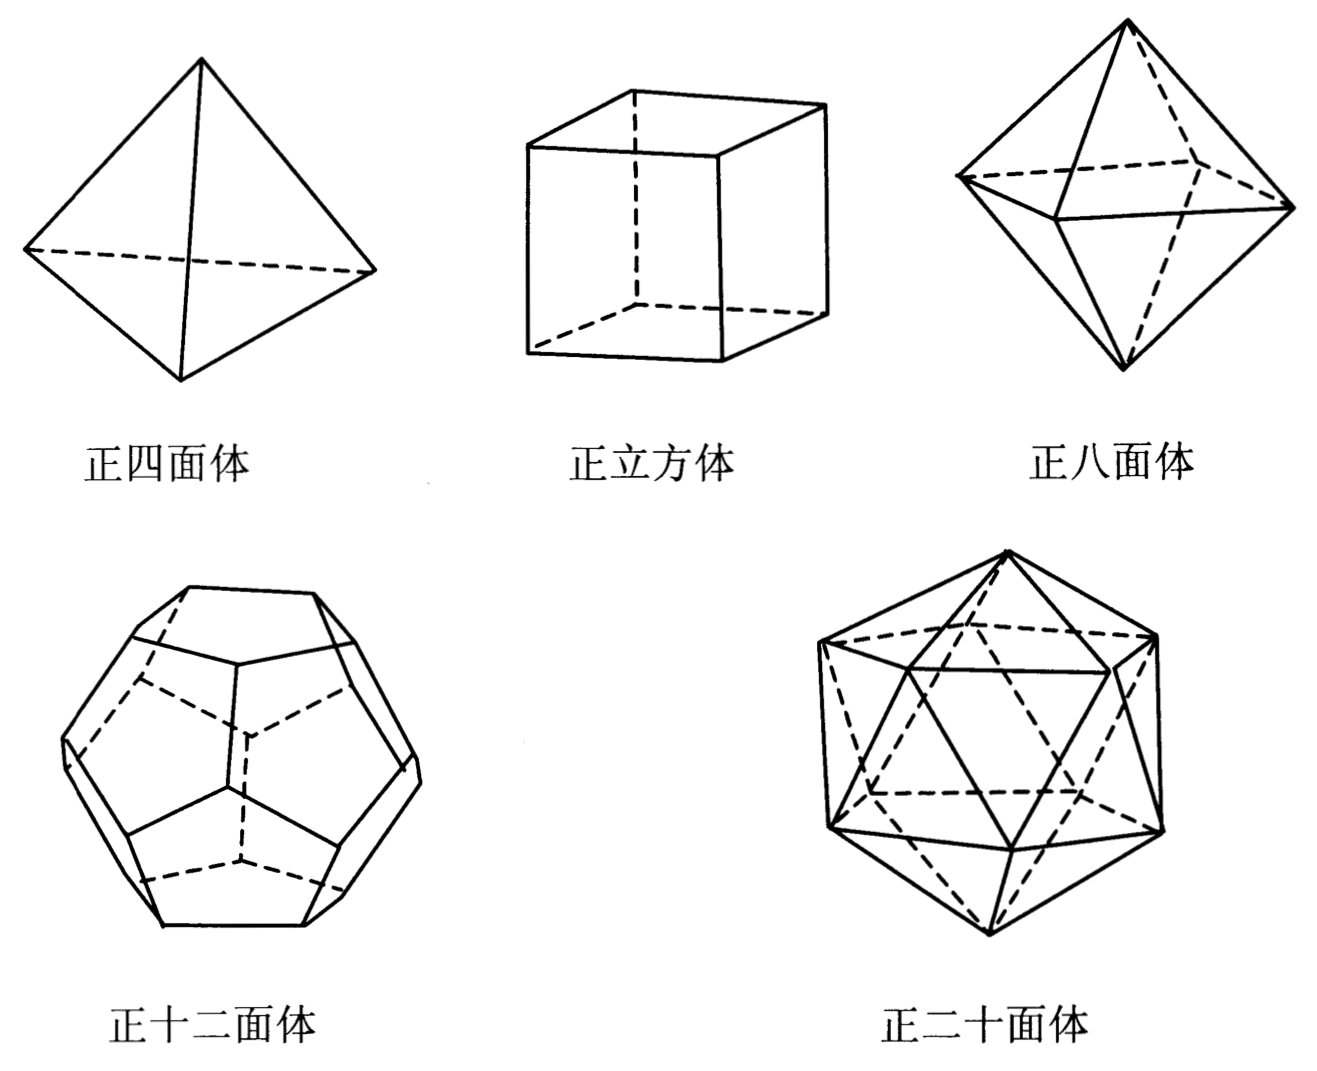
\includegraphics[width=0.65\linewidth]{figures/fig_1_118_1.png}\end{center}
\end{minipage}\par\vfill
\newpage
\noindent\begin{minipage}{\textwidth}\ProblemHeading{习题}{1.119}
设群 $G$ 在集合 $\Sigma$ 上的作用是传递的，且 $N\triangleleft G$。证明 $\Sigma$ 在 $N$ 作用下的所有轨道有相同的基数。
\end{minipage}\par\vfill
\noindent\begin{minipage}{\textwidth}\ProblemHeading{习题}{1.120（校订）}
设有限群 $G$ 作用在有限集合 $\Sigma$ 上，$t$ 为轨道数，$f(g)$ 为 $g\in G$ 的不动点数。证明 $\sum_{g\in G} f(g)=t\,|G|$。
\end{minipage}\par\vfill
\noindent\begin{minipage}{\textwidth}\ProblemHeading{习题}{1.121}
设 $p$ 是素数，$G$ 是有限 $p$ 群。证明 $G$ 的非正规子群个数是 $p$ 的倍数。
\end{minipage}\par\vfill
\newpage
\noindent\begin{minipage}{\textwidth}\ProblemHeading{习题}{1.122}
设 $G$ 是单群。若 $G$ 有一个真子群 $H$ 满足 $[G:H]\le4$，证明 $|G|\le3$。
\end{minipage}\par\vfill
\noindent\begin{minipage}{\textwidth}\ProblemHeading{习题}{1.123}
设无限群 $G$ 有一个有限指数的真子群 $H$。证明 $G$ 含有一个有限指数的真正规子群。
\end{minipage}\par\vfill
\noindent\begin{minipage}{\textwidth}\ProblemHeading{习题}{1.124}
证明一般线性群 $\mathrm{GL}(n,\mathbb C)$ 不含有限指数的真子群。
\end{minipage}\par\vfill
\newpage
\noindent\begin{minipage}{\textwidth}\ProblemHeading{习题}{1.125}
设 $|G|=2^n m$，其中 $m$ 为奇数。若 $G$ 含有一个 $2^n$ 阶元素，证明 $G$ 含有一个指数为 $2^n$ 的正规子群。
\end{minipage}\par\vfill
\noindent\begin{minipage}{\textwidth}\ProblemHeading{习题}{1.126}
求对称群 $S_3$ 的自同构群 $\operatorname{Aut}(S_3)$。
\end{minipage}\par\vfill
\noindent\begin{minipage}{\textwidth}\ProblemHeading{习题}{1.127}
设 $\alpha$ 是有限群 $G$ 的一个自同构，且对任意 $g\in G$，$g$ 与 $\alpha(g)$ 在 $G$ 中共轭。证明 $\alpha$ 的阶的每个素因子都整除 $|G|$。
\end{minipage}\par\vfill
\newpage
\noindent\begin{minipage}{\textwidth}\ProblemHeading{习题}{1.128}
设 $p$ 是 $|G|$ 的最小素因子。若 $A$ 是 $G$ 的 $p$ 阶正规子群，证明 $A\le C(G)$。
\end{minipage}\par\vfill
\noindent\begin{minipage}{\textwidth}\ProblemHeading{例题}{1.129（改写）}
举出拉格朗日定理的逆命题不成立的例子：证明 $30\mid |A_5|$，但 $A_5$ 没有 $30$ 阶子群。
\end{minipage}\par\vfill
\noindent\begin{minipage}{\textwidth}\ProblemHeading{例题}{1.130（改写）}
证明 $148$ 阶群不是单群。
\end{minipage}\par\vfill
\newpage
\noindent\begin{minipage}{\textwidth}\ProblemHeading{例题}{1.131（改写）}
证明 $56$ 阶群不是单群。
\end{minipage}\par\vfill
\noindent\begin{minipage}{\textwidth}\ProblemHeading{习题}{1.132}
设 $p$ 是有限群 $G$ 的阶的素因子。证明 $G$ 含有 $p$ 阶元素。
\end{minipage}\par\vfill
\noindent\begin{minipage}{\textwidth}\ProblemHeading{习题}{1.133}
设 $G$ 是 $n$ 阶群，$p$ 是 $n$ 的素因子。证明方程 $x^p=1$ 在 $G$ 中的解数是 $p$ 的倍数。
\end{minipage}\par\vfill
\newpage
\noindent\begin{minipage}{\textwidth}\ProblemHeading{习题}{1.134}
证明六阶非交换群在同构意义下只有 $S_3$。
\end{minipage}\par\vfill
\noindent\begin{minipage}{\textwidth}\ProblemHeading{习题}{1.135}
证明任意 $200$ 阶群都含有一个正规的西罗子群。
\end{minipage}\par\vfill
\noindent\begin{minipage}{\textwidth}\ProblemHeading{习题}{1.136}
对每个整除 $|S_4|$ 的素数 $p$，求 $S_4$ 的西罗 $p$ 子群个数。
\end{minipage}\par\vfill
\newpage
\noindent\begin{minipage}{\textwidth}\ProblemHeading{习题}{1.137}
求 $S_4$ 的自同构群 $\operatorname{Aut}(S_4)$。
\end{minipage}\par\vfill
\noindent\begin{minipage}{\textwidth}\ProblemHeading{习题}{1.138}
设 $N$ 是有限群 $G$ 的正规子群，$p$ 是素数。若 $p$ 与 $|G/N|$ 互素，证明 $N$ 包含 $G$ 的全部西罗 $p$ 子群。
\end{minipage}\par\vfill
\noindent\begin{minipage}{\textwidth}\ProblemHeading{习题}{1.139}
设 $G$ 是有限群，$N\triangleleft G$，$P$ 是 $G$ 的一个西罗 $p$ 子群。证明下列结论。
\SubQ{1}{$N\cap P$ 是 $N$ 的西罗 $p$ 子群。}
\SubQ{2}{$PN/N$ 是 $G/N$ 的西罗 $p$ 子群。}
\SubQ{3}{$N_G(P)N/N\cong N_{G/N}(PN/N)$。}
\end{minipage}\par\vfill
\newpage
\noindent\begin{minipage}{\textwidth}\ProblemHeading{习题}{1.140}
设 $P_1,\ldots,P_N$ 为有限群 $G$ 的全部西罗 $p$ 子群。若对任意 $i\ne j$，都有 $[P_i:P_i\cap P_j]\ge p^r$，证明 $N\equiv1\pmod{p^r}$。
\end{minipage}\par\vfill
\noindent\begin{minipage}{\textwidth}\ProblemHeading{习题}{1.141}
设 $G$ 是集合 $\Sigma$ 上的有限置换群，$P$ 是 $G$ 的西罗 $p$ 子群，$a\in\Sigma$。若 $p^m\mid |Ga|$，证明 $p^m\mid |Pa|$。
\end{minipage}\par\vfill
\noindent\begin{minipage}{\textwidth}\ProblemHeading{习题}{1.142}
设 $G$ 是集合 $\Sigma$ 上的有限置换群，$a\in\Sigma$，$P$ 是固定子群 $G_a$ 的西罗 $p$ 子群。令 $\Delta$ 是轨道 $Ga$ 中被 $P$ 的所有元素固定的点所成的集合。证明 $N_G(P)$ 在 $\Delta$ 上的作用是传递的。
\end{minipage}\par\vfill
\newpage
\noindent\begin{minipage}{\textwidth}\ProblemHeading{习题}{1.143}
设 $G$ 是 $24$ 阶群且 $C(G)=\{1\}$。证明 $G\cong S_4$。
\end{minipage}\par\vfill
\noindent\begin{minipage}{\textwidth}\ProblemHeading{习题}{1.144}
设 $P$ 是有限群 $G$ 的西罗 $p$ 子群，且 $N_G(P)\triangleleft G$。证明 $P\triangleleft G$。
\end{minipage}\par\vfill
\noindent\begin{minipage}{\textwidth}\ProblemHeading{例题}{1.145（改写）}
在以 $\{a,b,c\}$ 为基的自由群中完成下列计算。
\SubQ{1}{将 $(ab)(b^{-1}c)$ 约化。}
\SubQ{2}{将 $(ab)(b^{-1}a^{-1})$ 约化。}
\SubQ{3}{求 $a^3b^{-1}c$ 的逆。}
\end{minipage}\par\vfill
\newpage
\noindent\begin{minipage}{\textwidth}\ProblemHeading{例题}{1.146（改写）}
令 $F$ 是以 $\{a,b\}$ 为基的自由群，$K$ 是由 $a^3$ 和 $(ab)^2$ 正规生成的正规子群。写出商群 $F/K$ 的一个表现。
\end{minipage}\par\vfill
\noindent\begin{minipage}{\textwidth}\ProblemHeading{例题}{1.147（改写）}
设 $\varnothing$ 表示空的关系集。解释为什么群的表现 $\langle S\mid\varnothing\rangle$ 给出以 $S$ 为基的自由群。
\end{minipage}\par\vfill
\noindent\begin{minipage}{\textwidth}\ProblemHeading{例题}{1.148（改写）}
给出 $n$ 阶循环群 $\mathbb Z_n$ 的一个表现，并验证它确实定义了该群。
\end{minipage}\par\vfill
\newpage
\noindent\begin{minipage}{\textwidth}\ProblemHeading{例题}{1.149（改写）}
设 $D_n$（$n\ge3$）是正 $n$ 边形的对称群。以旋转一个顶点间隔和经过顶点的轴反射为生成元，写出 $D_n$ 的一个表现，并证明所列关系足以确定该群。
\end{minipage}\par\vfill
\noindent\begin{minipage}{\textwidth}\ProblemHeading{例题}{1.150（改写）}
设 $Q_8=\langle a,b\mid a^4=1,\ b^2=a^2,\ ba=a^3b\rangle$。在 $\mathrm{GL}(2,\mathbb C)$ 中取 $A=\begin{pmatrix}0&1\\-1&0\end{pmatrix}$、$B=\begin{pmatrix}0&i\\i&0\end{pmatrix}$，其中 $i^2=-1$。
\SubQ{1}{证明 $Q_8$ 的每个元素均可写为 $a^rb^s$，其中 $0\le r\le3$、$0\le s\le1$。}
\SubQ{2}{验证 $A,B$ 满足同样的关系，且八个矩阵 $A^rB^s$ 两两不同。}
\SubQ{3}{证明 $Q_8\cong\langle A,B\rangle$，且 $Q_8$ 是八阶非阿贝尔群。}
\end{minipage}\par\vfill
\noindent\begin{minipage}{\textwidth}\ProblemHeading{习题}{1.151}
设 $G=\langle g_1,\ldots,g_n\rangle$，$A\le G$ 的指数有限。证明 $A$ 可由至多 $2n[G:A]$ 个元素生成。
\end{minipage}\par\vfill
\newpage
\noindent\begin{minipage}{\textwidth}\ProblemHeading{习题}{1.152}
设 $n$ 为正奇数，证明 $D_{2n}\cong D_n\times\mathbb Z_2$。这里对 $m=1,2$，$D_m$ 也按表现 $\langle a,b\mid a^m=b^2=(ba)^2=1\rangle$ 定义。
\end{minipage}\par\vfill
\noindent\begin{minipage}{\textwidth}\ProblemHeading{习题}{1.153}
若 $n\ge3$，$A_n\times\mathbb Z_2$ 和 $S_n$ 是否同构？
\end{minipage}\par\vfill
\noindent\begin{minipage}{\textwidth}\ProblemHeading{习题}{1.154}
设 $G_1,G_2,G_3$ 是群。证明下列同构。
\SubQ{1}{$G_1\times G_2\cong G_2\times G_1$。}
\SubQ{2}{$(G_1\times G_2)\times G_3\cong G_1\times(G_2\times G_3)$。}
\end{minipage}\par\vfill
\newpage
\noindent\begin{minipage}{\textwidth}\ProblemHeading{习题}{1.155}
设 $G_1,\ldots,G_n$ 是群。证明以下结论。
\SubQ{1}{$C(G_1\times\cdots\times G_n)=C(G_1)\times\cdots\times C(G_n)$。}
\SubQ{2}{$G_1\times\cdots\times G_n$ 为阿贝尔群，当且仅当每个 $G_i$ 均为阿贝尔群。}
\end{minipage}\par\vfill
\noindent\begin{minipage}{\textwidth}\ProblemHeading{习题}{1.156}
设 $G_1,\ldots,G_n$ 是群，且 $N_i\le G_i$（$1\le i\le n$）。证明以下结论。
\SubQ{1}{$N_1\times\cdots\times N_n\le G_1\times\cdots\times G_n$。}
\SubQ{2}{$N_1\times\cdots\times N_n$ 是 $G_1\times\cdots\times G_n$ 的正规子群，当且仅当每个 $N_i$ 都是 $G_i$ 的正规子群。}
\SubQ{3}{若 $N_1\times\cdots\times N_n\triangleleft G_1\times\cdots\times G_n$，则 $\dfrac{G_1\times\cdots\times G_n}{N_1\times\cdots\times N_n}\cong(G_1/N_1)\times\cdots\times(G_n/N_n)$。}
\end{minipage}\par\vfill
\noindent\begin{minipage}{\textwidth}\ProblemHeading{习题}{1.157}
设 $H\le G=G_1\times\cdots\times G_n$。$H$ 是否一定可以写成 $H_1\times\cdots\times H_n$，其中 $H_i\le G_i$？
\end{minipage}\par\vfill
\newpage
\noindent\begin{minipage}{\textwidth}\ProblemHeading{习题}{1.158}
设 $G_1,G_2$ 是两个非阿贝尔单群，并将它们看作直积中的两个因子子群。证明 $G_1\times G_2$ 的非平凡真正规子群只可能是 $G_1$ 和 $G_2$。
\end{minipage}\par\vfill
\noindent\begin{minipage}{\textwidth}\ProblemHeading{习题}{1.159}
设 $\mathbb C^\times$ 为非零复数乘法群，$\mathbb R_{>0}^\times$ 为正实数乘法群，$\mathbb R$ 为实数加法群。证明 $\mathbb C^\times\cong\mathbb R_{>0}^\times\times(\mathbb R/2\pi\mathbb Z)$。
\end{minipage}\par\vfill
\noindent\begin{minipage}{\textwidth}\ProblemHeading{习题}{1.160}
设 $n_1,\ldots,n_r$ 是正整数。证明下列结论。
\SubQ{1}{$\mathbb Z_{n_1}\times\mathbb Z_{n_2}\cong\mathbb Z_{n_1n_2}$ 当且仅当 $(n_1,n_2)=1$。}
\SubQ{2}{若 $n_1,\ldots,n_r$ 两两互素，则 $\mathbb Z_{n_1}\times\cdots\times\mathbb Z_{n_r}\cong\mathbb Z_{n_1\cdots n_r}$。}
\end{minipage}\par\vfill
\newpage
\noindent\begin{minipage}{\textwidth}\ProblemHeading{习题}{1.161}
证明 $5\cdot7\cdot13$ 阶群一定是循环群。
\end{minipage}\par\vfill
\noindent\begin{minipage}{\textwidth}\ProblemHeading{习题}{1.162}
设 $G=G_1\times G_2$，$H\triangleleft G$，且 $H\cap G_i=\{1\}$（$i=1,2$）。证明 $H$ 是阿贝尔群。
\end{minipage}\par\vfill
\noindent\begin{minipage}{\textwidth}\ProblemHeading{习题}{1.163}
设 $G=G_1\times\cdots\times G_n$，各 $G_i$ 都有限，且当 $i\ne j$ 时 $|G_i|,|G_j|$ 互素。证明 $G$ 的任一子群 $H$ 都是子群 $H\cap G_i$（$i=1,\ldots,n$）的直积。
\end{minipage}\par\vfill
\newpage
\noindent\begin{minipage}{\textwidth}\ProblemHeading{习题}{1.164}
设 $G$ 是有限生成自由阿贝尔群，$\operatorname{rank}G=r$。若 $g_1,\ldots,g_n$ 构成 $G$ 的一组生成元，证明 $n\ge r$。
\end{minipage}\par\vfill
\noindent\begin{minipage}{\textwidth}\ProblemHeading{例题}{1.165（改写）}
分类所有 $1500$ 阶阿贝尔群。
\SubQ{1}{给出每个同构类型的初等因子。}
\SubQ{2}{将各初等因子分解改写为不变因子分解。}
\end{minipage}\par\vfill
\noindent\begin{minipage}{\textwidth}\ProblemHeading{习题}{1.166}
证明有限生成阿贝尔群 $G$ 为自由阿贝尔群，当且仅当 $G$ 的每个非零元素都具有无限阶。
\end{minipage}\par\vfill
\newpage
\noindent\begin{minipage}{\textwidth}\ProblemHeading{习题}{1.167}
设 $\mathbb Q_{>0}^\times$ 是正有理数乘法群。证明下列结论。
\SubQ{1}{$\mathbb Q_{>0}^\times$ 是自由阿贝尔群，全部素数构成它的一组基。}
\SubQ{2}{$\mathbb Q_{>0}^\times$ 不是有限生成群。}
\end{minipage}\par\vfill
\noindent\begin{minipage}{\textwidth}\ProblemHeading{习题}{1.168}
设 $\mathbb Q$ 是有理数加法群。证明下列结论。
\SubQ{1}{$\mathbb Q$ 不是自由阿贝尔群。}
\SubQ{2}{$\mathbb Q$ 的任意有限生成子群都是循环群，但 $\mathbb Q$ 本身不是循环群。}
\end{minipage}\par\vfill
\noindent\begin{minipage}{\textwidth}\ProblemHeading{习题}{1.169}
设 $A$ 是有限阿贝尔群。证明对 $|A|$ 的每个正因子 $d$，$A$ 都有一个 $d$ 阶子群和一个 $d$ 阶商群。
\end{minipage}\par\vfill
\newpage
\noindent\begin{minipage}{\textwidth}\ProblemHeading{习题}{1.170}
设 $H$ 是有限阿贝尔群 $A$ 的子群。证明 $A$ 有一个子群与 $A/H$ 同构。
\end{minipage}\par\vfill
\noindent\begin{minipage}{\textwidth}\ProblemHeading{习题}{1.171}
证明若有限阿贝尔群 $A$ 不是循环群，则存在素数 $p$，使得 $A$ 有一个子群同构于 $\mathbb Z_p^2$。
\end{minipage}\par\vfill
\noindent\begin{minipage}{\textwidth}\ProblemHeading{习题}{1.172（校订）}
设 $m,n$ 为正整数，$mn>1$。证明下列结论，其中 $(m,n)$ 为最大公因数，$[m,n]$ 为最小公倍数。
\SubQ{1}{若 $(m,n)=1$，则 $\mathbb Z_m\oplus\mathbb Z_n$ 的不变因子为 $\{mn\}$。}
\SubQ{2}{若 $(m,n)>1$，则 $\mathbb Z_m\oplus\mathbb Z_n$ 的不变因子为 $\{(m,n),[m,n]\}$。}
\end{minipage}\par\vfill
\newpage
\noindent\begin{minipage}{\textwidth}\ProblemHeading{习题}{1.173}
求 $\mathbb Z_2\oplus\mathbb Z_9\oplus\mathbb Z_{35}$ 的初等因子和不变因子。
\end{minipage}\par\vfill
\noindent\begin{minipage}{\textwidth}\ProblemHeading{习题}{1.174}
设 $p$ 是素数。求 $\mathbb Z_{p^3}\oplus\mathbb Z_{p^2}$ 的 $p^2$ 阶子群个数。
\end{minipage}\par\vfill
\noindent\begin{minipage}{\textwidth}\ProblemHeading{习题}{1.175}
证明非零复数乘法群 $\mathbb C^\times$ 的每个有限子群都是循环群。
\end{minipage}\par\vfill
\newpage
\noindent\begin{minipage}{\textwidth}\ProblemHeading{习题}{1.176}
设 $p$ 是素数，$G$ 是 $n$ 个 $p$ 阶群的直和。求 $G$ 的极大子群个数。
\end{minipage}\par\vfill
\noindent\begin{minipage}{\textwidth}\ProblemHeading{习题}{1.177}
设 $G,A,B$ 均为有限阿贝尔群。若 $G\oplus A\cong G\oplus B$，证明 $A\cong B$。
\end{minipage}\par\vfill
\noindent\begin{minipage}{\textwidth}\ProblemHeading{例题}{1.178（改写）}
在 $D_4=\langle a,b\mid a^4=b^2=1,\ ba=a^{-1}b\rangle$ 和 $Q_8=\langle a,b\mid a^4=1,\ b^2=a^2,\ ba=a^{-1}b\rangle$ 中，分别求 $a^ib^j$（$0\le i\le3,\ 0\le j\le1$）的阶，并说明为什么 $D_4$ 与 $Q_8$ 不同构。
\end{minipage}\par\vfill
\newpage
\noindent\begin{minipage}{\textwidth}\ProblemHeading{例题}{1.179（改写）}
设 $T=\langle a,b\mid a^6=1,\ b^2=a^3,\ ba=a^{-1}b\rangle$。在 $S_3\times\mathbb Z_4$ 中取 $A=((123),\alpha^2)$、$B=((12),\alpha)$，其中 $\alpha$ 是用乘法记号书写的 $\mathbb Z_4$ 的生成元。
\SubQ{1}{证明 $T$ 的每个元素都可写成 $a^ib^j$，其中 $0\le i\le5$、$0\le j\le1$。}
\SubQ{2}{验证 $A,B$ 满足 $T$ 的定义关系，并证明它们生成一个 $12$ 阶子群。}
\SubQ{3}{证明 $T\cong\langle A,B\rangle$，并用元素阶比较 $D_6,A_4,T$ 的同构类型。}
\end{minipage}\par\vfill
\noindent\begin{minipage}{\textwidth}\ProblemHeading{习题}{1.180}
分别求 $D_4$、$Q_8$ 的中心 $C(D_4)$、$C(Q_8)$。
\end{minipage}\par\vfill
\noindent\begin{minipage}{\textwidth}\ProblemHeading{习题}{1.181}
证明 $Q_8$ 的每个子群都是正规子群。
\end{minipage}\par\vfill
\newpage
\noindent\begin{minipage}{\textwidth}\ProblemHeading{习题}{1.182}
分别确定 $18$ 阶群和 $20$ 阶群的全部同构类型。
\end{minipage}\par\vfill
\noindent\begin{minipage}{\textwidth}\ProblemHeading{习题}{1.183}
设 $p,q$ 为素数，$p<q$。证明每个 $pq$ 阶非阿贝尔群都有表现 $G=\langle a,b\mid a^p=b^q=1,\ a^{-1}ba=b^r\rangle$，其中 $r^p\equiv1\pmod q$、$r\not\equiv1\pmod q$，且 $p\mid(q-1)$。
\end{minipage}\par\vfill
\noindent\begin{minipage}{\textwidth}\ProblemHeading{习题}{1.184}
设 $p$ 为奇素数。证明每个 $p^3$ 阶非阿贝尔群都有下列两个表现之一。
\SubQ{1}{$\langle a,b\mid a^{p^2}=b^p=1,\ b^{-1}ab=a^{1+p}\rangle$。}
\SubQ{2}{$\langle a,b,c\mid a^p=b^p=c^p=1,\ ca=ac,\ cb=bc,\ ab=bac\rangle$。}
\end{minipage}\par\vfill
\newpage
\noindent\begin{minipage}{\textwidth}\ProblemHeading{例题}{1.185（改写）}
设 $D_n$（$n\ge3$）是正 $n$ 边形的对称群。构造 $D_n$ 的一个可解列，证明 $D_n$ 是可解群。
\end{minipage}\par\vfill
\noindent\begin{minipage}{\textwidth}\ProblemHeading{例题}{1.186（改写）}
设 $|G|=pq$，其中 $p>q$ 为素数。构造 $G$ 的一个可解列，证明 $G$ 是可解群。
\end{minipage}\par\vfill
\noindent\begin{minipage}{\textwidth}\ProblemHeading{习题}{1.187}
证明 $S_3$ 和 $S_4$ 都是可解群。
\end{minipage}\par\vfill
\newpage
\noindent\begin{minipage}{\textwidth}\ProblemHeading{习题}{1.188}
设 $p,q,r$ 是素数，可以有相同的取值。证明 $pqr$ 阶群都是可解群。
\end{minipage}\par\vfill
\noindent\begin{minipage}{\textwidth}\ProblemHeading{习题}{1.189}
设 $f:G\to A$ 是群同态，且 $A$ 是阿贝尔群。证明 $G'\le\ker f$，其中 $G'$ 是 $G$ 的换位子群。
\end{minipage}\par\vfill
